% -*- eval: (activate-input-method 'spanish-postfix); -*-
\documentclass[12pt,a4paper]{report}

\usepackage[margin=2.5cm]{geometry}
\usepackage{tikz}
\usepackage{circuitikz}
\usepackage{cite}
\usepackage{amssymb}
\usepackage{amsfonts}
\usepackage{hyperref}
\usepackage{amsmath}
\usepackage{graphicx}
\usepackage{indentfirst} 
\usepackage{xfrac}
\usepackage{xcolor}
\usepackage{calc}


\title{Fundamentos Matematicos de la Criptografia: Un resumen}
\author{Tomas Fabrizio Orsi}
\date{\today}

\begin{document}

\maketitle
\tableofcontents

\newcommand{\li}[1]{\ensuremath{\mathcal{{#1}}}}
\newcommand{\mat}[1]{\ensuremath{\mathbb{{#1}}}}
\newcommand{\rarrow}{\rightarrow}
\newcommand{\darrow}{\downarrow}
\newcommand{\xor}{\oplus}
\newcommand{\claude}{Claude ``La Cabra'' Shannon }
\newcommand{\alicebob}{
\begin{center}
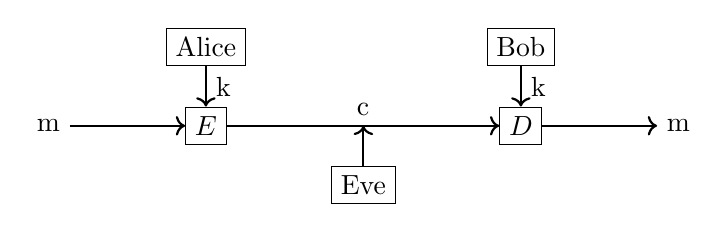
\begin{tikzpicture}
  \node[draw, rectangle] (encript) at (0,0) {$\li{E}$};
  \node[draw, rectangle] (decript) at (4,0) {$\li{D}$};

  \node[draw, rectangle] (alice) at (0,1) {$\text{Alice}$};
  \node[draw, rectangle] (bob) at (4,1) {$\text{Bob}$};
  \node[draw, rectangle] (eve) at (2, -0.75) {$\text{Eve}$};

  \draw[->, thick] (encript) -- node[above] {c} (decript);

  \node[draw=none, rectangle] (mensajeEntrada) at (-2,0) {m};
  \draw[->, thick] (mensajeEntrada.east) -- (encript.west);

  \node[draw=none, rectangle] (mensajeSalida) at (6,0) {m};
  \draw[->, thick] (decript.east) -- (mensajeSalida.west);

  \draw[->, thick] (alice.south) -- node[right] {k} (encript.north);
  \draw[->, thick] (bob.south) -- node[right] {k} (decript.north);

  \draw[->, thick] (eve.north) -- (2, 0);

\end{tikzpicture}
\end{center}
}
\newcommand{\esquema}{$(\li{P}, \li{C}, \li{K}, \li{E}, \li{D}, \li{R})$ }

\newcommand{\divides}{\mid}
\newcommand{\ndivides}{\nmid}
\newcommand{\modulo}[1]{\; \bmod \; {{#1}}}
\newcommand{\cuerpo}[1][n]{\ensuremath{\sfrac{\li{Z}}{#1 \li{Z}}}}
\newcommand{\divent}{\backslash}
\newcommand{\orden}[1]{\ensuremath{\text{ord}({#1})}}


\part{Fundamentos matemáticos}

\chapter{Preludio}

\section{Glosario}

\begin{itemize}

\item Plaintext($\li{P}$): Mensaje sin encriptar
\item Mensaje($\li{M}$): Mensaje sin encriptar, sinónimo de plaintext
\item Cifrado($\li{C}$): Mensaje encriptado
\item Alfabeto($\li{A}$) : Conjunto de todas las letras que componen el plaintext y el cifrado

\end{itemize}


\section{Criptogramas Históricos}

\subsection{Cifrado de Cesar}
Cifrado usado por Julio Cesar para encriptar mensajes. En teoría usado en la guerra de las Galias.


El alfabeto consiste en todas las letras del alfabeto latino:
$
\mathcal{A} = \{ A, B, \dots, Z \}
$

El esquema de encriptación consiste en reemplazar cada letra con la letra que le sigue 3 veces (loopeando en la Z). Esto se escribe: $ m \rarrow m + 3$. Mas precisamente, es: $m + 3 \mod 26$ ya que el modulo tiene esta logica de ``looping''.

Para desencriptar, se hace lo opuesto, se \textit{resta} a las letras del cifrado: $ c \rarrow c + 3$


\subsection{Cifrados por módulo generico}

El cifrado de Cesar canónico es solo un subcaso del cifrado por modulo 26.

En generico, lo podemos plantear como: $c  = m + k \mod 26$ (el módulo 26 nace de que el abecedario tiene 26 letras).

\subsubsection{¿Como obtener el K de un cifrado arbitarario?}

Estos cifrados son bastante débiles porque rapidamente podes obtener el $k$ usado, solo tenes que probar todos los $k$ posibles, los cuales no son muchos, ya que solo pueden ir de 1 a 26 (debido al tamño del abecedario)
Ademas, no hace falta probar todos los numeros con todo el mensaje. Ya con pocas letras podes darte cuenta que el mensaje no tiene sentido.

\subsection{Cifrado por permutación}

Este cifrado es como la versión ``genérica'' de todos los cifrados.
Mi mensaje original decimos que es $m = m_1 || m_2 \dots || m_l$, donde $m$ es el mensaje entero, $m_i$ es cada caracter de ese mensaje y $||$ es el operador concatenar.


Mi funcion de cifrado es una función biyectiva e inversible $f$, que se la aplico a cada caracter de $m$ para obtener $c$, es decir: $c = f(m_1) || f(m_2) || \dots || f(m_l)$.
Como la función es inversible, para desencriptar el mensaje, le aplico $f^{-1}$ a todos los $c$ para obtener mis $m$s originales:
$m = f^{-1}(c_1) || f^{-1}(c_2) || \dots || f^{-1}(c_l)$.

\subsubsection{Propiedades}
¿Cuantas funciones biyectivas puedo tener para un alfabeto de n elementos?
La respuesta es: $n!$. ¿Por qué? Porque son todas las \textbf{permutaciones} del alfabeto original.
La primera letra puede mapearse a todos los elementos del alfabeto ($n$ posibilidades), la segunda puede mapearse a todos los elementos excepto el que usó la primera letra ($n -1$ posibilidades), y así sucesivamente. Multiplicando todas las posibilidades te queda $n!$. ¡Magia!

\subsubsection{Crackeo via Análisis de frecuencia}

¿Como haces para \href{https://youtu.be/oozWzypjmqk}{crackear} un cifrado?

Por fuerza bruta no vas a tener buenos resultados porque son $n!$ posibilidades, vas a estar un rato \textbf{largo}.

Se crackea haciendo análisis de frecuencia.
Para esto, tenes que hacerte un compilado del idioma en el que está escrito el mensaje original. Una vez tengas ese compilado, analizas cual es la frecuencia de cada una de las letras de tu idioma y te armas una tablita.

Después, haces esa misma tabla de frecuencia con los caracteres del mensaje cifrado.

Una vez que tengas las dos tablas, podes ver que letra del cifrado tiene una frecuencia similar a la del idioma original. Lo mas probable es que sean la misma letra, y si no, va a ser una de las letras con frecuencia similar.

Esto tambien implica, que cuanto mas largo sea el mensaje cifrado, mas susceptible a este tipo de crackeo es. ¿Por qué? Porque cuantas mas letras cifradas haya, mas la distribución se van a parecer.

\subsection{Nomenclador}
Es un cifrado que busca evitar caer en el análsis de frecuencia. Consiste en hacer una correspondencia que va de símbolos (incluso varios a la vez) a palabras. Incluso puede saltear palabras.

Sin embargo, este metodo tambien es vulnerable al analisis de frecuencia.

\subsection{Vigenere a.k.a ``cifrado indecifrable''}
Es como una especie de cifrado de Cesar en paralelo.

Tenes un llave $k$ que es $k = (r_1, r_2, \dots r_n)$. Esto representa un \textbf{conjunto de indices}, es decir, la primera letra va usar $r_1$ como pad, despues la segunda $r_2$ y asi.

Tu mensaje $m$ que se \textbf{parte de una forma diferente}. $m = m_1 || m_2 || \dots m_n$, pero \textbf{cada $m_i$ tiene una longitud de $n$ caracteres}, no 1 como era en Cesar.

Entonces, ¿como funciona?. Cada $m_i$ es un conjunto de caracteres de longitud menor o igual a $n$ (siendo $n$, como dijimos antes, la longitud de la llave).

Entonces, vos para encriptar $m_i$ tenes que encriptar cada caracter de $m_i$ con el offset corresponspondiente de la llave $k$, es decir:
$$
c_i[j] = m_i[j] + k[j] \mod 26
$$
Siendo $m_i[j]$ el $j$-ésimo caracter del conjunto de letras $i$-ésimo. Mismo $c_i[j]$.

Ejemplo: Dado $k = (3,1,11,3)$.

\begin{itemize}
\item $m_1 = ABAB \rarrow c_1 = DCRE $
\item $m_2 = CEB \rarrow c_2 = FFS $ \footnote{En los casos donde la palabra es mas corta que la llave, solo usas hasta el indice que necesitas}
\end{itemize}

Todo es un golazo, pero Baggage y Co decifraron que esto tambien es vulnerable al analisis de frecuencia.

\subsection{OTP: One tine pad}
\label{otp}
La madre de todos los cypers.

Aca, el alfabeto $\li{A}$ dejan de ser las letras de la A a la Z y pasan a ser bits, $1$ o $0$. Los mensajes están codificados como tiras de estos bits: $m = b_1 || b_2 || b_3$.

Y, notoriamente, ya no uso suma con módulo para encriptar, sino que uso el operador XOR $\xor$. $c = m \xor k$. Esto significa que necesito tener una llave de igual longitud que el mensaje

Una propiedad piola del $\xor$ es que tambien es su propio inverso, para desencriptar el mensaje, hago $m = c \xor k$.

Lo importante, es que \textbf{siempre necesito una llave distinta, no puedo repetir llave.} Si repito, perdí seguridad.

¿Como hacian para conseguir esto? Generaban aleatoriamente \footnote{Generar cualquiercosa aleatoriamente no era tribial en esta epoca. Tampoco hoy en dia. feojfeoqjfoqjefjfpq. Ponele, ahi toqué el teclado a lo loco y aprete principalmente teclas en el centro del teclado. Conclusion: Es facil introducir un sesgo u no darse cuenta.} llaves de gran longitud y la almacenaban en cuadernos.
Luego enviaban, en aviones, estos cuadernillos con llaves a las personas que se tenían que comunicar e iban usando una página por vez.

\subsubsection{Problemas}
El OTP es bastante sólido, pero tiene problemas

\begin{itemize}
  \item{La generacion aleatoria de llaves no es trivial}
  \item{En algun momento, te vas a quedar sin paginas. ¿Que haces ahi? No podes reutilizar. Tenes que re-imprimir un nuevo cuaderno}
  \item{Distribucion: Distribuir el cuaderno no es ni facil ni barato. Lo hacian por avion.}
\end{itemize}

\section{Principios de la criptografia}

La criptografia esta principalmente centrada en afrontar 3 pilares centrales de la encriptacion de mensajes.

\begin{itemize}
  \item{\textbf{Integridad:} No poder alterar el mensaje original}
  \item{\textbf{Autenticidad:} Poder saber que quien dice haber enviado un mensaje es realmente quien dice ser}
  \item{\textbf{No repudiabilidad:} La propiedad de no poder negar haber recibido un mensaje que realmente recibiste}
\end{itemize}

\section{Esquema de encriptacion}

Un esquema de encriptacion gneerico se puede entender con el siguiente grafico.

\begin{center}
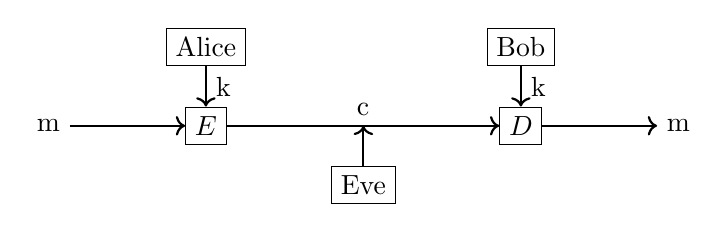
\begin{tikzpicture}
  \node[draw, rectangle] (encript) at (0,0) {$\li{E}$};
  \node[draw, rectangle] (decript) at (4,0) {$\li{D}$};

  \node[draw, rectangle] (alice) at (0,1) {$\text{Alice}$};
  \node[draw, rectangle] (bob) at (4,1) {$\text{Bob}$};
  \node[draw, rectangle] (eve) at (2, -0.75) {$\text{Eve}$};

  \draw[->, thick] (encript) -- node[above] {c} (decript);

  \node[draw=none, rectangle] (mensajeEntrada) at (-2,0) {m};
  \draw[->, thick] (mensajeEntrada.east) -- (encript.west);

  \node[draw=none, rectangle] (mensajeSalida) at (6,0) {m};
  \draw[->, thick] (decript.east) -- (mensajeSalida.west);

  \draw[->, thick] (alice.south) -- node[right] {k} (encript.north);
  \draw[->, thick] (bob.south) -- node[right] {k} (decript.north);

  \draw[->, thick] (eve.north) -- (2, 0);

\end{tikzpicture}
\end{center}

Donde Alice encripta el mensaje usando su llave $k$, obtenido el cipher $c$. Este se lo envia a Bob por un canal donde Eve puede verlo. Luego Bob desencripta el mensaje usando la llave $k$.

Esto es un esquema de encriptacion simétrico, en uno asimetrico las llaves son distintas.

\section{Historia: Maquina enignma}

La maquina enigma fue una maquina de encriptacion desarrollada por una empresa alemana en ``tiempos de paz''.
Despues, cuando estalla la guerra, el ejercito aleman la incorpora añadiendole sus propias modificaciones.

Esta maquina consistia en una serie de rotores que iban girando cada vez que una tecla se apretaba y una configuracion inicial de dichos rotores. Cada rotor servía de nivel de indireccion, entonces cuantos mas rotores, mas dificil era saber la configuracion inicial de la maquina. La gracia de este mecanismo era complicar el analisis de frecuencia.


Tenía una serie de problemas, algunos sociales y otros mecánicos.

Problemas sociales:
\begin{enumerate}
  \item{Era comercial: Al ser comercial, habia muchos maquinas disponibles lo cual facilitaba su estudio}
  \item{Se leakearon cuadernos: alguien que labura en la fabrica donde se producian regaló cuadernos con llaves.}
  \item{El manual de instrucciones tenia mucha informacion. Primero, describia como se podia usar la maquina y segundo tenia un ejemplo de la maquina en funcionamiento.}
\end{enumerate}

Problemas mecánicos:
\begin{itemize}
  \item{El teclado estaba ordenado alfabeticamente \footnote{El profesor dijo que esto era un problema, yo no entendí por que}}
  \item{La configuracion de la maquina la enviaban dos veces al dia por si una se perdia. Esto les termino jugando en contra.}
  \item{El azar de la configuracion lo determinaba una persona. Era muy suceptible a introducir sesgo}
  \item{\textbf{Ninguna letra se podía encriptar como sí misma.} Esta era la mayor falla.}
  \item{Todos los mensajes seguían un formato estandarizado (ej, primero heil Hitler, despues el clima, despues novedades, etc). Esto facilitó el análisis de frecuencia.}
\end{itemize}

\subsection{Los polacos olvidados}

Usando el manual de instrucciones de la maquina original, un grupo de matematicos polacos lograron decifrar como funcionaba la maquina mucho antes de la guerra y de Turing.

Su trabajo y hallazgos se lo dieron a los Franceses e Ingleses. La maquina de Turing en gran parte consistia de una automatizacion del trabajo de los polacos.



\section{Teoría de la informacion}
\claude formaliza matematicamente la comunicacion

Define formalmente un esquema de encriptación: $(\li{P}, \li{C}, \li{K}, \li{E}, \li{D}, \li{R})$, siendo:

\begin{itemize}
    \item{$\li{P}:$ Plaintext }
    \item{$\li{C}:$ Cipertext }
    \item{$\li{K}:$ Llave (key)}
    \item{$\li{E}:$ Funcion de Encriptacion}
    \item{$\li{D}:$ Funcion de Desencriptacion}
    \item{$\li{R}:$ Fuente de aleatoriedad usada para generar la llave.}
\end{itemize}

\alicebob

\subsection{Cesar como esquema de encriptacion}
Usando esta notacion podemos escribir al esquema de cesar:

\begin{itemize}
\item{$ \li{P} = \{\text{alfabeto} \} = \li{C}$.}
\item{$\li{E} = m + 3 \mod 26$ }
\item{$\li{D} = c - 3 \mod 26$ }
\end{itemize}
No tiene llaves $\li{K}$ per se.

\subsection{Postulado de Kerckoff}
El esquema/algoritmo/function no es un secreto, eventualmente se hace público o lo decifran. Lo \textbf{unico} secreto, son las llaves.

\section{Criptografia moderna}
Hay dos formas de entender cuando comienza la: o en 1949 con la teoría de información de shannon o en en 1978 con los esquema de llave pública.

La criptografia moderna tiene una fuerte base matematica. Consiste en definiciones, diseñar esquemas usando dichas definciones y luego modelar las capacidades del adversario.

\subsection{Problemas de la criptografia}
Los problemas principales de la criptografia son 3:
\begin{itemize}
  \item{Generar: Es super jodido generar llaves realmente aleatorias}
  \item{Distribuir: Es super jodido distribuir llaves sin que el enemigo las intercepte.}
  \item{Guardar: Guardar no es trivial. ¿Como las cuidas a que se arruinen? ¿Como evitas que las roben?}
\end{itemize}

\section{Teoremas de Shannon}
\claude da dos definiciones zarpadas y mas importante aun \textbf{postula que son iguales}, uno implica el otro.

\subsection{Perfect secrecy}
\label{perfect-secrecy}
Dice que un esquema \esquema  es perfect secrecy si cumple que la probabilidad de que el mensaje contenga $m_i$ dado que salio $c_i$ sea la \textbf{misma probabilidad} a que tenga $m_j$ (que sean independientes). Es decir, que el cipher \textbf{no me de informacion sobre el mensaje original.}

Matematicamente, esto se denota asi:
$$
\mat{P}[ M = m | \li{D}(K, M) = c ] = \mat{P}[M=m]
$$
Siendo $\li{D}$ la función de desencriptación

\subsection{Perfect indistinguishibility}

Esta otra definicion me dice que dado el criptograma $c$, yo no puedo saber si $c$ viene de $m_1$ o de $m_2$. Es decir, que no haya ``sesgo'' o ``pista'' sobre su origen.

Matematicamente:

$$
\mat{P}[\li{E}(K, m_1) = c] = \mat{P}[\li{E}(K, m_2) = c]
$$


\subsection{Teorema de Shannon sobre OTP}
Postula que \nameref{otp} es \nameref{perfect-secrecy} sii se usa adecuadamente.

La criptografia moderna busca a conseguir OTPs practicos.

\subsubsection{Demostración perfectly indistinguishable}
$$
\mat{P}[\li{E}_K(m_1) \footnote{La notacion $E(k,m)$ y $E_k(m)$ son notaciones distintas para decir que se encripta $m$ con la funcion de encriptacion $E$ y la llave $k$} = c] = \mat{P}[\li{E}_K(m_2) = c] 
$$

Dado el mesnaje $m_1$, hay una unica llave que encripta $m_1$ a $c$, y es $k$, $c = m_1 \xor k$.
¿Cual es la probabilidad de obtener un $c$ dado? $\mat{P}[\li{E}_K(m_1) = c]$. Es la misma probabilidad de que vos elijas la llave que te va a desencriptar $c$.

¿Cual es esa probabilidad? Es la probabilidad de probar todas las llaves una a una.
Entonces, ¿cuantas llaves hay? $2^n$ ($2$ porque las palabras son bits $1$ o $0$ y $n$ porque es la longitud del mensaje). Entonces, ala probabilidad de adivinar la llave es $\frac{1}{2^n}$. Ademas, cuanto mas largo el mensaje, menos chance hay.

\subsection{Teorema de Shannon sobre que requiere perfect secrecy}
Para que un esquema sea perfectly secret, \textbf{requiere} que se cumpla:
$$ | P | \leq | K|$$

Es decir, necesitamos que haya mas o igual llaves ($K$) que mensajes ($P$).

La explicacion del profe no la entendi asique fui al paper de \claude \cite{shannon1949}. Por suerte, está bastante intuitivo.

\claude dice, vos necesitas que haya tantos $\li{C}$ como $\li{M}$. ¿Por que? Y necesariamente necesitas que todos los mensajes puedan mapearse a todos los ciphers encriptados. Sino fuese asi, podes decir ``Ah, tengo $C_1$ y yo se que tiene que ser o $M_1$ o $M_2$, pero ninguno mas''. Eso \textbf{no} nos sirve.

Necesitamos algo asi:
\begin{center}
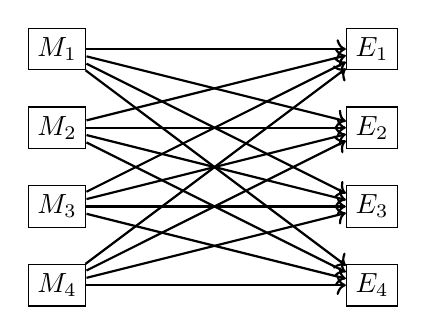
\begin{tikzpicture}
  \node[draw, rectangle] (M1) at (0,3) {$M_1$};
  \node[draw, rectangle] (M2) at (0,2) {$M_2$};
  \node[draw, rectangle] (M3) at (0,1) {$M_3$};
  \node[draw, rectangle] (M4) at (0,0) {$M_4$};

  \node[draw, rectangle] (E1) at (4,3) {$E_1$};
  \node[draw, rectangle] (E2) at (4,2) {$E_2$};
  \node[draw, rectangle] (E3) at (4,1) {$E_3$};
  \node[draw, rectangle] (E4) at (4,0) {$E_4$};

  \draw[->, thick] (M1) to (E1);
  \draw[->, thick] (M1) to (E2);
  \draw[->, thick] (M1) to (E3);
  \draw[->, thick] (M1) to (E4);

  \draw[->, thick] (M2) to (E1);
  \draw[->, thick] (M2) to (E2);
  \draw[->, thick] (M2) to (E3);
  \draw[->, thick] (M2) to (E4);

  \draw[->, thick] (M3) to (E1);
  \draw[->, thick] (M3) to (E2);
  \draw[->, thick] (M3) to (E3);
  \draw[->, thick] (M3) to (E4);

  \draw[->, thick] (M4) to (E1);
  \draw[->, thick] (M4) to (E2);
  \draw[->, thick] (M4) to (E3);
  \draw[->, thick] (M4) to (E4);

\end{tikzpicture}
\end{center}

ENTONCES, como necesitamos que todo se pueda mapear a todo y tengo una única funcion $\li{E}$, \textbf{necesariamente} necesito que haya tantas llaves $k$ como palabras $m$.

\section{Modelos de ataque}
¿Como logra Eve interactuar con el esquema?

\subsection{Blackbox model}
Solo se ve lo que entra y/o sale, no se puede acceder a la implementacion física

\subsubsection{Ciphertext only attack}
Pasivo. El atacante solo lee los ciphertext. Esto es lo que uno asume siempre.
\subsubsection{Known plaintext}
Pasivo. El atacante tiene una lista de de pares $(m_i, c_i)$. Es decir, tiene algunas preimagenes. Es pasivo porque no busco obtener los pares, los obtuvo.
\subsubsection{Chosen plaintext attack}
Activo. El atacante tiene la capacidad de encriptar mensajes de su elección y desencriptarlos.
\subsubsection{Chosen ciphertext attack}
Este no lo entendi.

\chapter{Teoría de numeros basicos}
\section{Teorema fundamental del álgebra}
Dado un $n \in \li{N}$, existe un unico conjunto ordenado de primos $p_1, p_2, \dots p_l$ y potencias naturales $e_1, e_2, \dots e_l$ tales que:
$$
n = \prod_{i = 1}^{l} p_i^{e_i}
$$

Esto es una manera fachera de decir: Todos los numeros se pueden \textbf{factorizar} como una potencia de potencias primos.

\section{Algoritmo de división}
Dados $a, b$ existe un único $q$ y $r$ con $0 \leq r \leq |b|$ tal que $a = b \cdot q + r$.

Llamamos $q$ a cociente y a $r$ restante.

\section{Divisibilidad}
Decimos que $a$ e divisible por $b$ si $r=0$ cuando $a= b \cdot q + 0$.

$$
b \divides a \rarrow \text{a es divisible por b}
$$
$$
b \ndivides a \rarrow \text{a no es divisible por b} \\
$$

Una manera de recordar el orden es leerlo como \textbf{$a$ divide a $b$}.

\subsection{Resto}
$$
r_a(b) \rarrow \text{Resto de dividir a por b}
$$

\section{Divisores de un numero}
Los divisores de un numero $a \in \li{Z}$ es el conjunto de los numeros que $Div(a) = \{ b \in \li{Z} : b \divides a \}$
Ejemplo:
$$
Div(12) = \{ \pm 1, \pm 2, \pm 3, \pm 4. \pm 6, \pm12 \}
$$

Este conjunto de numeros es un conjunto \textbf{finito}. Tambien hay que notar que los divisores son siempre el par de un numero y el mismo nergado. Asique solo nos vamos a centrar en los positivos.
Estrictamente, existe $Div^+(a)$ que refiere estrictamente a los divisores positivos de $a$. Para el curos $Div^+(a) \approx Div(a)$

\section{Numero primo}
Definimos numero primo a un numero que solo tiene como divisor a sí mismo. Otra forma de definirlo es $| Div(n_p) | = 4$ (sí mismo y 1, positivo y negativo).

\subsection{Problemas y propiedades}
\begin{enumerate}
  \item{Dado un $n \in \li{N}$ decidir si es primo es dificil. Hay que chequear sus divisores, lo cual require un algoritmo computacionalmente jodido.}
  \item{Dado un $n \in \li{N}$ compuesto \footnote{Compuesto = No primo} hallar un divisor de $n$ también es jodido. Una vez encontrado un divisor, chequearlo es sencillo. Se \textit{cree} que \textbf{no} hay un algoritmo en tiempo polinomial que me dice si se puede factorizar.}
\end{enumerate}


\subsection{Teorema de Euclides}
Es una de las primeras demostraciones de que hay infinitos numeros primos.

La idea es probarlo por el absurdo. Supongamo que los numeros primos son finitos y digamos que son $\li{P} = \{ p_1, p_2, p_3, \dots \}$. Ahora, agarro y los multiplico todos juntos y le pongo $m$, en criollo: $\prod_{i = 1} p_i$. Y despues le sumo uno a ese $m$, llamemoslo $m'$.

Y $r_{p_i}(m') = 1$, entonces ningun numero de $\li{P}$ divide a $m'$, entonces $m'$ es primo!

Ergo, hay un absurdo, ergo son infinitos.

\subsection{Super Teorema de Euler}
Dado $\li{P}$, la suma:
$$
\sum \frac{1}{p_i} = \infty
$$
\subsection{Teorema del numero primo}
Busca contestar, ¿cuantos primos hay menores o iguales a un numero $x$?
$$
| \{p \in \li{P} : p \leq x \} | \approx \frac{x}{\log(x)}
$$

\subsection{Conjetura del numero primo}
Postula que existen infinitos primos tal que $p + 2$ tambien es primo.

\subsection{Conjetura de los primos de Gilmain}
Postula que existen infinitos primos tal que $\frac{p - 1}{2}$ tambien es primo.

\subsection{Criba de Erastótenes}
Es uno de los primeros métodos para ahallar primos.
Arrancas anotando los numeros de izquierda a derecha, hasta el numero que vos querés averiguar. Vas tachando los numeros que son multiplos del numero actual, despues aumentas en uno.

Conseguis los primos, pero es exponencial en tiempo y lineal en memoria.

\subsection{Busqueda de primos $\sqrt{n}$}

No hace falta hacer $n$ pruebas para ver los primos. Solo necesitas $\frac{\sqrt{n}}{2}$.

\begin{itemize}
  \item{El $\sqrt{n}$ viene de TODO}
  \item{El dividido $2$ es porque no necesito probar los pares}
\end{itemize}

\section{Divisores comunes}
Entendemos a los divisores comunes entre dos numeros $a$ y $b$ como los divisores que son tanto de $a$ como de $b$

En español:
$$
Div(a, b) = Div(a) \land Div(b)
$$

\subsection{Máximo común divisor: MCD}
Es el divisor común mas grande entre los dos.
Se lo anota como $(a : b)$

\section{Co-primos}
Dos $a$ y $b$ son co-primos si no tienen divisores comunes entre sí.
$(a : b) = 1$

% \subsection{¿Cómo hallar co-primos?}
\subsection{$Div^+(a,b) = Div^+(b, a - q \cdot b)$}

\section{Algoritmo de Euclides}
Manera gauchita de encontrar el máximo común divisor ($r$) entre dos numeros.

Arranca con el siguiente facto:
$$
a, b \in \li{N}, (a : b)  = (b, r_b(a))
$$

¿Que significa esto? Que si es muy complicado encontrar el MCD de dos numeros, puedo simplemente tratar de hallar el MCD de uno de esos numeros con el resto de la division de estos dos.
¿Y que gano con eso? Y, un montón! Porque se me simplifica la complejidad en cada iteración del problema.

En a los sumo \textbf{$b$ pasos}, llegas a $r$.


\subsection{Algoritmo de Euclides extendido}

Dados $a, b \in \li{Z}$, existe $k, l \in \li{Z}$, tal que:
$$
(a: b) = k \cdot a + l \cdot b
$$

El MCD es una combinacion lineal entera de $(a, b)$. Ademas, es la \textbf{menor} combinación lineal positiva entra $a$ y $b$.

\subsubsection{Algoritmo de Euclides de Coprimos}

Si $a, b$ son co-primos, entonces:
$$
1= a \cdot k + b \cdot l
$$

¿Qué quiere decir esto? Que si el algoritmo me dá como resultado 1, \textbf{son coprimos} y por lo tanto no tienen divisores comunes.
Si me da cualquier otro número, significa que no son coprimos y que ese número que me dió es el mcd.

\subsubsection{Aplicación de Euclides de Coprimos}
Si $p$ primo. Si $p | a \cdot b \rarrow p | a \lor p | b$


Ejemplo:


$(3 \divides 18) = (3 \divides 6 \cdot 4) \rarrow (3 \divides 6)$

\chapter{Aritmetica modular}

\section{Relación de equivalencia}
Si $\mat{A}$ es un conjunto, una relacion de equivalencia en $\mat{A}$ es un subconjunto $\mat{R} \subset A x A$ tal que:
\begin{enumerate}
    \item{Tiene que ser reflexiva: $\forall a \in \mat{A} (a,a) \in \mat{R}$. Es decir, todos los elementos están relacionados con sí mismo}
    \item{Tiene que ser simétrica: Si $(a, b) \in \mat{R} \rarrow (b, a) \in \mat{R}$.}
    \item{Tiene que ser transitiva: Si $(a,b) \in \mat{R} \;\land\; (b,c) \in \mat{R} \;\rarrow\; (a,c) \in \mat{R}$}
\end{enumerate}

Cuando $\mat{R}$ es de equivalencia, se suele escribir: $a \equiv_{\mat{R}} b$.

\section{Clase de equivalencia}
Decimos que la clase de equivalencia es el conjunto $\bar{a} \footnote{Solo pongo el gorro en este capitulo, a partir de ahora lo voy a poner sin el gorro} = \{ b \in \mat{R}  : a \equiv_{\mat{R}}b\}$.

\subsection{Propiedades}
En la clase de equivalencia de $\bar{a}$. Si $(a, b) \in \mat{A}$:
\begin{itemize}
  \item{$a \in \bar{a}$}
  \item{$b \in \bar{a} \rarrow a \in \bar{b}$}
  \item{O bien $\bar{a} = \bar{b}$ o bien $\bar{a} \land \bar{b} = \varnothing$. Es decir, o son iguales o son disjuntos.}
\end{itemize}

\subsection{La relacion de equivalencia como partición de A}
Una relacion de equivalencia $\mat{R}$ en un conjunto $\mat{A}$ es una \textbf{particion} de $\mat{A}$.
Todas relaciones de equivalencia unidas forman $\mat{A}$.

\section{Aritmética Modular}
$\sfrac{\li{Z}}{n \li{Z}}$ se define como la relacion de equivalencia: 
$$
(a \equiv b) (\modulo{n})
$$
Dado $n \in N$ y si $n \divides a - b$.

\subsection{Valores que la toman}
Los numeros que forman parte de la relacion de equivalencia de $\bar{m}$ son:
$$
\{ \bar{m} = m + n \cdot k, k \in Z \}
$$

\subsection{Clases de equivalencia en la relacion}
Hay $n$ clases de equivalencia en la relacion, todas disjuntas.

$$
\modulo{n}  = \{ \bar 0, \bar 1 \dots \overline{n-1} \}
$$

Cada uno de los numeros que ponemos en el conjunto se los llama ``representante''. Esto es porque todos los valores de clase representan al mismo conjunto, por convención se pone el ``mas bajo positivo''.


Los representantes son los \textbf{restos} de dividir por $n$.

\subsection{Operaciones}
Se definen las siguientes operaciones en $\sfrac{\li{Z}}{n \li{Z}}$.
\subsubsection{Suma}
Se define
$$\bar a + \bar b = \overline{a + b}$$

Como:
$$
a + b = r_n(a+b)
$$

Propiedades:
\begin{itemize}
    \item{Hay un neutro: $\bar a + \bar 0 = \bar a$ \footnote{Con la notacion de modulo esto es $a + 0 \equiv a \modulo{n}$}}
    \item{Es conmutativo: $\bar a + \bar b = \bar b + \bar a$}
    \item{Tiene un inverso aditivo: $\bar a + - \bar a = \bar 0$. El inverso de un numero es $n-a$.}
    \item{Es asociativo: $\bar a + (\bar b + \bar c) = (\bar a + \bar b) + \bar c$}
\end{itemize}

\subsubsection{Producto}
Se define
$$\bar a \cdot \bar b = \overline{a \cdot b}$$

Como:
$$
a \cdot b = r_n(a \cdot b)
$$

Propiedades:
\begin{itemize}
  \item{Si $a$ es multiplo de $n$, la tabla de $a$ es $a$ y $0$.}
  \item{Si $a$ es coprimo de $n$, la tabla de $a$ es completa: todos los valores de la relación de equivalencia.}
\end{itemize}

\subsubsection{Exponenciar}
Se define
$$\bar a^l = a \cdot a \cdot a \cdot a \dots_{\text{l veces}} $$

\subsection{Teorema ecuaciones modulares con producto}
\label{sec:teorema-coprimos-ecuaciones}
En \cuerpo, la ecuacion $$a \cdot x \equiv 1 \modulo{n}$$ tiene solución si y solo si $(a : n) \equiv 1$. Es decir, solo si $a$ y $n$ son co-primos.


Si $(a:n) \neq 1 \rarrow a \cdot x = 1$ no tiene solucion. Además, en este caso, $a$ es un divisor de cero en \cuerpo; osea que $a \cdot b \equiv 0 \modulo{n}$.

\section{Unidades}

Las unidades de \cuerpo es el conjunto
$$
U(\cuerpo) = \{a \in \cuerpo \; \exists \; x ; \; a \cdot x \equiv 1 \; (\modulo{n})\}
$$

\subsection{Teorema coprimos}
Por \nameref{sec:teorema-coprimos-ecuaciones}

$$
U(\cuerpo) = \{a \in \cuerpo \; ; (a: n) \equiv 1\}
$$

\subsection{Teorema multiplos de unidades}
Si $a, b \in U(\cuerpo) = a \cdot b \in U(\cuerpo)$

Osea, $ U(\cuerpo), \cdot) $ forma un grupo.


\section{Funcion de Euler $\varphi$}

Se define $$\varphi(n) = | U(\cuerpo)|$$

Es decir, se define como la cantidad de elementos en las unidades de $\cuerpo$.

\subsection{Calculo de $\varphi$}
Sabiendo factorizar.

\begin{enumerate}
    \item{Si $p$ es primo, $\varphi(p) = p - 1$}
    \item{Si $n = p^r \rarrow \varphi(n) = p^r - p^{r-1} =p^{r-1} \cdot (p-1)$}. Ejemplo: $\varphi(8) = \varphi(2^3) = 2^3 - 2^2 = 4$
    \item{Si $(a:b) = 1 \land \varphi(a \cdot b) \rarrow \varphi(a \cdot b) =  \varphi(a) \cdot \varphi(b) $}
\end{enumerate}

\section{Teorema Euler - Fermat}
Tiene dos partes

\subsection{Teorema Fermat}
Si $p$ primo y $(a : p) \equiv 1$, entonces:
$$
a^{\varphi(p)} = a^{p-1} \equiv 1 \ \modulo{p}
$$

Además, si $p$ primo, $a ^ p \equiv a \ \modulo{p}$.

\subsection{Teorema Euler}
Si $(a : n) = 1$, entonces:
$$a^{\varphi(n)} \equiv 1 \ \modulo{n}$$

\section{Teorema Chino del resto}
\subsection{Teorema: Unica solución ecuación $a \cdot x = b$.}

La ecuación:
$$
a \cdot x = b \ \modulo{n}
$$

tiene una solución $0 \leq x <n$ cuando $(a:n) = 1$.


La solución es $a^{-1} \cdot b \ \modulo{n}$. Siendo $a^{-1}$ el inverso de $a$, es deir el numero $c$ en \cuerpo tal que $a \cdot c \equiv 1$

\subsection{Teorema: Solución de ecuación $a \cdot x = b$ cuando $(a : n) \neq 1$.}

Siendo $(a: n)= d$, entonces $a \cdot x = b \ \modulo{n}$ tiene solución si y solo si $d | b$. En este caso, la ecuacion se tiene que ``co-primar'':
$$
\frac{a}{d} \cdot x = \frac{b}{d} (\modulo{\frac{n}{d}})
$$

Esta nueva ecuación tiene la misma solución que la ecuacion original.

\subsection{Teorema: Definicion de resolver una ecuación de congruencia lineal}
Para resolver una ecuacion del tipo $a \cdot x \equiv b \modulo{n}$, tiene dos soluciones posible:
\begin{itemize}
  \item{No tiene solucion}
  \item{O se reduce a una ecuación alternativa: $x \equiv b' \modulo{n'}$}
\end{itemize}

\subsection{Teorema chino del resto: Aplicación}

$$
\begin{cases}
x \equiv b_1 \pmod{m_1} \\
x \equiv b_2 \pmod{m_2} \\
\quad\vdots \\
x \equiv b_l \pmod{m_l}
\end{cases}
$$

Con $m_1, m_2, \dots m_l$ coprimos dos a dos. Tiene una unica solución, $0 \leq x \leq \prod m_i$

\subsubsection{Solución}
Sea $$M = \prod^l m_i$$

Definimos,
$$
M_j = \frac{M}{m_j} = \prod^l_{i = 1, i \neq j} m_i
$$

Esto hace que $(M_j : m_j) = 1$, es decir que todos son coprimos entre sí. Esto produce que exista un unico $y_j$ tal que:
$$
y_j \cdot M_j \equiv 1 \modulo{m_j}
$$

Entonces:
$$
\sum_{i=1}^l y_j \cdot M_j \equiv \modulo{m_j}
$$

Además:
$$
\sum_{i=1}^l b_i \cdot y_i \cdot M_i \equiv b_j \modulo{m_j}
$$

Y, la solucion buscada, $x$, es la primera parte:
$$
x = \sum_{i=1}^l b_i \cdot y_i \cdot M_i
$$

OJO, a veces esa $x$ no es la menor representate, entonces
$$
x \equiv x_0 \modulo{\prod m_i}
$$

\chapter{Algebra abstracta}
\section{Grupos}
Es un conjunto \li{G} con operación ``por'' $\cdot$ tal que:
\begin{enumerate}
  \item{$a \cdot (b \cdot c) = (a \cdot b) \cdot c$}
  \item{Existe identidad $e$ tal que: $a \cdot e = e \cdot a = a$}
  \item{Existe inverso multiplicativo $a^{-1}$: $a \cdot b = b \cdot a = 1_{\li{G}}$}
\end{enumerate}
\subsection{Grupos abelianos}
Decimos que un grupo ademas es abeliano si tambien vale la propiedad conmutativa:
$$
a \cdot b = b \cdot a
$$

\subsection{Subgrupos}
\label{sec:subgrupos}


Los unicos subgrupos en $(\cuerpo, +)$ son:
$$
\cuerpo[m], \; m | n
$$

Si $n$ es primo, solo hay un subgrupo: sí mismo

Ejemplo: En $\cuerpo[6] = \{ 0, 1, 2, 3, 4, 5 \}$
\begin{itemize}
\item $\cuerpo[0] = \{0 \}$
\item $\cuerpo[2] = \{0, 3 \}$
\item $\cuerpo[3] = \{0, 2, 4 \}$
\end{itemize}

\subsection{Teorema de Lagrange}
\label{sec:teorema-langrange}

Si \li{G} es un grupo finito y $\li{H} \in \li{G}$  (es decir es un subgrupo), el \textbf{tamaño de \li{H} divide al tamaño de \li{G}}.

Esto normalmente se usa al reves: vos te fijas el tamaño de \li{G} y te fiijas cuales son los posibles tamaños de los grupos. Ejemplo: $|\li{G}| = 32$ los subgrupos pueden tener tamaño: 1, 2, 4, 8, 16, 32.

\subsection{Orbita}
\label{sec:orbita}

Si \li{G} es un grupo finito, $g \in \li{G}$ es el subgrupo generado por: $\{g^0, g^1, g^2, \dots, g^l\}$ y se lo escribe:
$$
<g>
$$

\subsubsection{Orden}
El tamaño de este grupo $g$ se llama orden de g, \orden{g}.
\begin{itemize}
\item Por Lagrange: $\orden{g} \; | \; \; |\li{G}|$
\item $\orden{g} = \min_{i \in N} \{ g^i = 1 \}$
\end{itemize}

\subsection{Grupo Ciclico}
\label{sec:grupo-ciclico}

\li{G} es cíclico si existe $<g> = \li{G}$

Se dá que las unidades de $n$ (osea cuando $(m:n) = 1$):
$$
\cuerpo[n] = <m>
$$

\paragraph{Observacion:}

Un grupo cíclico es abeliano.


\subsubsection{Ejemplo}

En $(\cuerpo[12], +)$ los generados son $U(\cuerpo[12])$: $<1>, <5>, <7>, <11>$.

Los otros forman sub-grupos de a partes:
$$
\begin{aligned}
<2> = <10> &= \{0, 2, 4, 6, 8, 10 \} \\
<3> = <9>  &= \{0, 3, 6, 9 \} \\
<4> = <8>  &= \{0, 4, 8 \} \\
<6> &= \{0, 6 \} \\
\end{aligned}
$$

\subsection{Teorema de los subgrupos similares}
\label{sec:grupos-similares}

En \cuerpo, para cada divisor $d$ de $n$, hay un \textbf{unico subgrupo de tamaño $d$} en \cuerpo, que ``es como'' \cuerpo[d]. 


Un posible generador de dicho grupo, aunque no el unico, es: $\frac{n}{d}$.

\subsection{Suma de grupos}
\label{sec:suma-grupos}

Si $\li{G}_1$ y $\li{G}_2$ son grupos $\li{G}_1 \xor \li{G}_2$ es un nuevo grupo con elementos siendo pares ordenados:
$$
(g_1, g_2) \; ; g_1 \in \li{G}_1 \land g_2 \in \li{G}_2
$$

Y la suma se entiende como:
$$
(g_1, g_2) + (h_1, h_2) = (g_1 + h_1, g_2 + h_2) 
$$

\subsection{Teorema chino del resto en terminos de grupos}
\label{sec:chino-grupo}

Si $$m = \prod^l_{i = 1} m_i\; ; (m_i: m_j) = 1$$ entonces:
fjlafja 

\begin{itemize}
\item $\cuerpo[m] \approx \xor \footnote{Esto es como la ``xoreada'', xor-eo todo} \cuerpo[m_i]$
\item $U(\cuerpo) \approx \xor U(\cuerpo[m_i])$
\item $\varphi(m) = \prod \varphi(m_i)$
\end{itemize}

Esta idea es biyectiva: puedo formar sub-grupos que $\xor$-eados formen todo \cuerpo y dado un \cuerpo puedo hallar sub-grupos que lo formen.

Ir de los subgrupos al grupo es mas dificil que ir del grupo a los sub-grupos.

% \subsubsection{Ejemplo}

% $$
% \cuerpo[6] = \{ 0, 1, 2, 3, 4, 5 \}
% $$

% ¿Como puedo descomponerlo en sub-grupos? Primero, por Lagrange, tengo que buscar los divisores de 6: 2, 3.  Con esto se que los subgrupos van a tener tamaño 2 y 3.

\subsection{Teorema de estructura para grupos abelianos finito}

Si $\li{G}$ es abeliano finito, entonces:
$$
\li{G} = \xor^l \li{G}_{p_i} ; \; i \neq j
$$
siendo $p$ primo y
$$
G_{p_i} = \xor^{l_i}_{j = 1} \; \cuerpo[p_i^{e_j}] \; ; e_j \in N
$$

\paragraph{Observaciones:}

\begin{itemize}
\item $p_i^{e_j} \; | \; |\li{G}|$
\item Propiedad importante: $|\li{G}_{p_i}|  = \prod p_i^{e_j} = p_i^{\sum e_j}$
\end{itemize}

Que significa la segunda? Que si agarro $|\li{G}|$ y lo factorizo en numeros primos, puedo hallar los posibles grupos descompiendo cada una de las potenicas.

\section{Anillos}
Decimos que un anillo
$$
(\li{A}, +, \cdot)
$$ es anilli si y solo si:
\begin{itemize}
\item $(A, +)$ es abeliano
\item Es distributivo con el producto: $ a \cdot (b + c) = a \cdot b + a \cdot c$
\item Es asociativo con el producto: $a \cdot (b \cdot c) = (a \cdot b) \cdot c$
\item (Opcional) puede tener identidad si $a \cdot 1 = 1 \cdot a$.
\item (Opcional) puede ser conmutativo con el producto: $a \cdot b = b \cdot a$.
\end{itemize}

\subsection{Unidades en anillo conmutativo y con identidad}

$$
U(\li{A}) = \{ a \cdot b = 1 \; ; a \in \li{A} \; \land \; b \in \li{A}  \}
$$

Es decir, los elementos inversibles de \li{A}.

\subsubsection{Unidades de polinomio}

En general, siendo $\li{A}[x]$ los polinomios en \li{A}:
$$
U(\li{A}[x]) = U(\li{A})
$$

\part[Criptografia Simétrica]{Criptografia Simétrica
  \parbox{0.8\textwidth}{\normalsize\normalfont
En estos esquema de encriptación, Alice y Bob acuerdan una llave previamente (normalmente la misma para ambos). Hoy en dia es comu que se haga un intercambio de llaves de forma asimetrica y despues en la comunicacion se hace simetrica. Hay ``dos'' grandes tipos: Cifrado de flujo, cifrado por bloque y los Modos de Operación (subtipo de los cifrado por bloque).}}


\chapter{Stream cipher o Cifrado de flujos}
La gracia de este tipo de ciphers es generar tiras de bits largas que parezcan aleatorias a partir de tiras de bits cortas usando tecnicas de PRNG: Pseudo Random Number Generator.

\section{Pseudo Random Number Generator}
Un Pseudo Random Number Generator es un generador de numberos que los genera de forma \textit{simil} aleatoria. Lo simil viene del hecho que la gracia de estos es que el resultado que producen se puede reproducir consistentemente dado la misma semilla. Esta reproducibilidad de hecho es un plus.

La gracia de esto no es solo que sea estadisticamente aleatorio, sino, mas importantemente, que no se pueda predecir los siguientes bits a partir de los primoeros n bits.

\subsection{Definicion matematica}

Definimos a \li{G} como un deterministic polinomial time algorithm; tal que $\forall n \in \mat{N}, \forall s \in \{0,1\}^n \rarrow G(s)$ es una tira de bits de longitud $\textit{l}(n)$.

Ahora, decimos que \li{G} es un PRNG si:
\begin{itemize}
  \item{$\forall \textit{l}(n) > n$. Esto es, se dá una expansión.}
  \item{$\forall D$ existe $\li{N}(n)$ tal que: $|P(D(G(s)) = 1) - P(D(r) = 1) | \leq \li{N}(n)$}
\end{itemize}

Con
\begin{itemize}
  \item{$D$ una funcion probabilistica polinomial time}
  \item{$\li{N}$ funcion negligible}
  \item{$r$ elegido uniforme $\{0, 1\}^{\li{l}(n)}$}
\end{itemize}

\section{Algoritmo Blum -- Blum -- Schob}
Sea $M = p \cdot q$ con $p, q$ primos. $p \equiv 3(4)$.

Definimos la secuencia formada por el siguiente algoritmo:
$$
x_{n + 1} = x_n^2 ; \mod {M}
$$

Con $x_0 \neq 0,1,p,q$.
La tira de bits resultante se obtiene a partir de la paridad del numero que se obtuvo en la iteracion: Si obtuviste un par va 0, impar va 1.
Si factorizar es dificil, BBS es un PRNG.

El problema que tiene este metodo es que usa muchos bits para generar los numeros pero despues solo se fija la paridad. Es muy caro para lo que usa para generar la secuencia de bits.

\section{Linear Feedback Shift Register}
Circuito electrico hecho con flip flops.
\subsection{Flip-flop}
Un flip flop es un componente electico. Es la unidad basica de memoria. Conceptualmente, es una ``cajita'' asociada a un reloj (o ``clock'' in inglish). En un tick $x$ se le da un input 0 o 1, al tick  $x + 1$ transmite el tick como output. En el tick $x + 2$ no dá mas output (a menos que se e haya dado un input antes).

\begin{center}
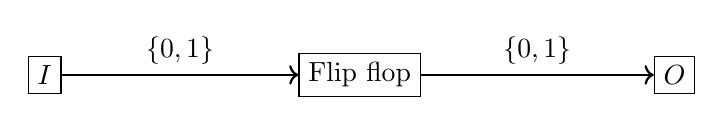
\begin{tikzpicture}
  \node[draw, rectangle] (flipflop) at (0,0) {Flip flop};
  \node[draw, rectangle] (input) at (-4,0) {$\li{I}$};
  \node[draw, rectangle] (output) at (4,0) {$\li{O}$};
  \draw[->, thick] (input) -- node[above] {$\{0, 1\}$} (flipflop);
  \draw[->, thick] (flipflop) -- node[above] {$\{0, 1\}$} (output);
\end{tikzpicture}
\end{center}

\subsection{Representación circuital}

Los LFSR son cadenas de flip flops conectados a compuertos XOR.

\begin{center}
\begin{circuitikz}
  \node[draw] (ff1) at (0,0) {$FF_{n}$};
  \node[draw] (xor1) at (1,2) {$\oplus$};
  \draw[<-] (ff1.west) -- ++(-1,0) |- (xor1.west);
  \draw (1,0) to[nos] (xor1.south);
  \draw[->] (-2,0) to (-1.5,0);

  \node[draw] (ff2) at (2,0) {$FF_{n-1}$};
  \node[draw] (xor2) at (3,2) {$\oplus$};
  \draw (xor1.east) to (xor2.west);
  \draw (3,0) to[nos] (xor2.south);
  \draw (ff1.east) to (ff2.west);

  \node at (4,1) {$\cdots$};
  \draw (xor2.east) to (4,2);
  \draw (ff2.east) to  (3,0);

  \node[draw] (ff3) at (6,0) {$FF_2$};
  \node[draw] (xor3) at (5,2) {$\oplus$};

  \draw (xor3.west) to (4,2);
  \draw (ff3.west) to  (3,0);
  \draw (5,0) to[nos] (xor3.south);

  \node[draw] (ff4) at (8,0) {$FF_1$};
  \node[draw] (xor4) at (7,2) {$\oplus$};
  \draw (7,0) to[nos] (xor4.south);
  \draw (ff3.east) to (ff4.west);
  \draw (xor3.east) to (xor4.west);

  \draw [->] (ff4.east) to (10,0);

  \draw (9,0) -- ++(0,2) to (xor4.east);
\end{circuitikz}
\end{center}

$P_i$ son las llaves electricas. Si $P_i$ vale 0, entonces está abierta, si vale 1 está cerrada. El estao de la llave se determina en la entrada y es conocido.

El estado que entra al circuito es: $S_n = \sum p_i \cdot S_i$.

Despues de un tick de reloj, el estado de los flip-flops va a cambiar. Como la cantidad de estados es finita, despues de una cantidad $v$ de operaciones, el estado del circuito va a volver al estado original. Esa cantidad $v$ la llamamos \textbf{período}. \\
El periodo $v$ es, \textit{a lo sumo} , $2^n - 1$, sin embargo no todos los circuitos llegan a ese máximo; pero existe una forma de formarlos.

\paragraph{Ejemplo}

\begin{center}
\begin{circuitikz}

  % Xors
  \node[draw] (xor1) at (1,2) {};
  \node[draw] (xor2) at ($(xor1) + (2,0)$) {$\oplus$};

  % Flip Flops
  \node[draw] (ff1) at (0,0) {$FF_{1}$};
  \node[draw] (ff2) at ($(ff1) + (2,0)$) {$FF_{2}$};
  \node[draw] (ff3) at ($(ff2) + (2,0)$) {$FF_{3}$};

  % Cables entre Flip Flops
  \draw (ff1.east) to (ff2.west);
  \draw (ff2.east) to (ff3.west);

  % Cables entre XORs
  \draw (xor1.east) to (xor2.west);

  % Cables entre XORs y Flip Fops
  \draw ($(ff3) + (-1,0)$) to (xor2.south);

  % Cables especiales
  %% Cables finales. Loop y flecha
  \draw ($(ff3) + (1,0)$) -- ++(0,2) to (xor2.east);
  \draw[->] (ff3) to ($(ff3) + (2,0)$);
  %% Cable iniciales. Loop y flecha.
  \draw[<-] (ff1.west) -- ++(-1,0) |- (xor1.west);
  \draw[->] ($(ff1) + (-2,0)$) to ($(ff1) + (-1.5,0)$);
\end{circuitikz}
\end{center}

\begin{center}
\begin{tabular}{c|c|ccc}
Clock & $FF_2 = FF_1 \oplus FF_0$ & $FF_2$ & $FF_1$ & $FF_0$ \\
\hline
0 & ---              & \textcolor{red}{1} & \textcolor{red}{0} & 1 \\
1 & $0 \oplus 1 = $ \textcolor{green}{1} & \textcolor{green}{1} & \textcolor{red}{1} & \textcolor{red}{0} \\
2 & $1 \oplus 0 = 1$ & 1 & 1 & 1 \\
3 & $1 \oplus 1 = 0$ & 0 & 1 & 1 \\
4 & $1 \oplus 1 = 0$ & 0 & 0 & 1 \\
5 & $0 \oplus 1 = 1$ & 1 & 0 & 0 \\
6 & $0 \oplus 0 = 0$ & 0 & 1 & 0 \\
7 & $1 \oplus 0 = 1$ & 1 & 0 & 1 \\
\end{tabular}
\end{center}

\subsection{Linear Feedback Shift Register de período máximo}

Tenemos el $FF_n = \sum p_i \cdot FF_i$ que es el estado del circuito. A esto le vamos a aasociar el polinomio:
\begin{align*}
f &= x^n + \sum p_i \cdot x^i \in F_2[X] \\
f &= x^n + p_{n-1} x^{n-1} + p_{n-2} x^{n-2} \dots p_1 \cdot x + p_0
\end{align*}

Se ``ve'' que $p_0$ siempre tiene que ser 1, por que? Por que si $p_0$ fuese cero, habría una raiz trivial con x = 0, y \textbf{no} queremos eso.

\subsection{Representación matricial}
Al polinomio $f$ lo podemoms representar como una matriz llamada \textbf{``matriz compañera''}.

$$
A = \begin{bmatrix}
  0 & 1 & 0 & \dots & 0 \\
  0 & 0 & 1 & \dots & 0 \\
  \vdots \\
  p_0 & p_1 & p_2 & \dots & p_{n-1} \\
    \end{bmatrix}
$$

Esta matriz tiene:

\begin{itemize}
\item{La diagonal de identidad corrida en uno.}
\item{Los valores de todos los $p_i$ en la ultima fila.}
\end{itemize}

Con esta matriz, podemos plantear la transformación del estado los flipflops de esta forma:
$$
A \cdot \begin{bmatrix} FF_0 \\ FF_1 \\ \vdots \\ FF_{n-1} \end{bmatrix} = \begin{bmatrix} FF_1 \\ FF_2 \\ \vdots \\ FF_{n} \end{bmatrix}
$$

Acá se ve bien la idea del LFSR: Todos los flip flops desplazan su bit al siguiente flip flop, y el próximo ``nuevo'' estado se obtiene en $FF_n$. Tambien podemos elevar esta matriz a una potencia.

$$
A^j \cdot \begin{bmatrix} FF_0 \\ FF_1 \\ \vdots \\ FF_{n-1} \end{bmatrix} = \begin{bmatrix} FF_j \\ FF_{j + 1} \\ \vdots \\ FF_{j + n - 1} \end{bmatrix}
$$

\subsubsection{Propiedades}
\begin{itemize}
\item{El Determinante de $A$ es $p_0$, osea 1.}
\item{$A$ es inversible}
\item{El polinomio caracteristico de A se obtiene: $\chi_A = \det(\lambda \cdot I - A)$.}
\item{El polinomio minimal $m_A$ es el polinomio de menor grado tal que si yo reemplazo $x$ por $A$ en el polinomio me dá 0, es decir: $m_A(A) = 0$}
\item{En los LFSR, $m_A = \chi_A$}
\end{itemize}

\subsection{LFSR de polinomios irreducibles}
Si $f$ en $F_2[X]$ es \textbf{irreducible}, todo estado inicial tiene el \textit{mismo} periodo que es igual al orden de A. El orden de A es $l$ mínimo tal que $A^l = I$. Esto solo nos resuelve mitad del problema, ahora sabemos que si el polinomio original es irreducible todos los estados tienen el mismo periodo. Ahora, como logramos garantizar que el dicho periodo sea el \textbf{máximo}.

La respuesta nos lo dan los cuerpos de Galois. $F_q$ siendo $q = 2^n$ y siendo $U(F_q)$ son sus unidades. Se da lo siguiente (ojo):
\begin{enumerate}
  \item $U(\mathbb{F}_q)$ es un grupo cíclico de $q-1$ elementos.

  \item $\mathbb{F}_q \cong \mathbb{F}_2[X]/(f)$, con $f \in \mathbb{F}_2[X]$, siempre y cuando $f$ sea irreducible de grado $n$ (con $q = 2^n$).

  \item $\mathbb{F}_q$ es el cuerpo de descomposición de $X^q - X$.

  \item Como $U(\mathbb{F}_q) \cong \mathbb{Z}/(q-1)\mathbb{Z}$, tiene $\varphi(q-1)$ generadores.

  \item Los generadores de $U(\mathbb{F}_q)$ se llaman \textbf{``Elementos primitivos''} y hay $\varphi(q-1)$.

  \item Los polinomios de grado $n$ que se anulan en elementos primitivos se llaman \textbf{``Polinomios primitivos''} y hay $\dfrac{\varphi(q-1)}{n}$.

  \item Hay tablas de polinomios primitivos en $\mathbb{F}_2[X]$ que tienen pocos XOR (computacionalmente ``livianos'').
\end{enumerate}

\subsection{LFSR de polinomios primitivos}
El LFSR asociado a un $f \in F_2[X]$ con grado $n$ tiene un periodo de $2^n-1$ si y solo si $f$ es un polinomio primitivo.

Una propiedad muy interesante y piola es que \textbf{primitivo implica irreducible}.
Esto responde la pregunta que haciamos antes: \textbf{solo necesitas un polinomio primitivo}. Entonces ahora ya sabemos como hacer circuitos piolas,  entendiendo por piola:

\begin{itemize}
\item Todos los $S_n$ tienen el mismo periodo
\item Dicho periodo es el maximo de $2^n -1$ siendo $n$ el grado del polinomio
\end{itemize}

\subsection{LFSR de PPI}

El problema que tienen los LFSR de PPP\footnote{PPI significa polinomio primitivo irreducible} es que son lineales: dada una cantidad larga de
ouput uno puede obtener la seed original.

En este contexto, la ``seed'' del LFSR es el estado inicial que se le entrega al
circuito (los primeros ``$n$'' bits que mandamos). Es por esto que todas las
implementaciones de LFSR tratan de introducir algún tipo de no linealidad
(\nameref{sec:a51}, \nameref{sec:trivium}, \nameref{sec:chacha},
\nameref{sec:salsa20}).

\section{A5/1}
\label{sec:a51}

\section{Trivium}
\label{sec:trivium}

\section{Cha-cha}
\label{sec:chacha}

\section{Salsa 20}
\label{sec:salsa20}

\appendix
\chapter{Practicas}

\section{Encontrar representante de número negativo}
Digamos que tenes un número negativo y querés hallar a qué representante pertenece.

Si es un número que está en el rango de la relación de equivalencia, haces la cuenta y listo.
Ejemplo:
$$
-3 \modulo{4} 
$$

Siendo chiquito, hago: $4 - 3 = 1$, entonces
$$
-3 \modulo{4} = 1 \modulo{4} 
$$


Ahora, digamos que tenes un numero grande como:
$$
-97 \modulo{7}
$$

Aca, ¿que haces?

\subsection{Hallas el congruente negativo más cercano}
Te fijas cual es el resto del número negativo en versión positiva. Es decir, haces:
$$
97 \divent 7 = 13
$$
Pero, no llego a $97$ con $7 \cdot 13$, \textbf{tengo un resto}. Para hallarlo hago: $97 - (7 * 13) = 6$.
Esto quiere decir que:
$$
97 = 7 \cdot 13 + 6
$$

Osea que:
$$
-97 \modulo{7} = -6 \modulo{7}
$$

\subsection{Hallas el representante canónico}
Ahora, solo tenés que restar el número que encontraste por el modulo, eso te dá el representante canónico.

$$
7 - 6 = 1
$$

Osea que:
$$
-97 \modulo{7} = 1 \modulo{7}
$$

\subsection{Chequeo}
Para chequear que está bien podes fijarte si $1$ y $-97$ pertenecen a la misma familia.

Primero, buscas el múltiplo necesario de restas:

$$
\left\lceil \frac{97}{7} \right\rceil\footnote{este es el simbolo de ceiling, aka "redondeá para arriba} = 14
$$

Con esto, te fijas si $1$ menos $7$ veces $14$ es $-97$.
$$
1 - 14 \cdot 7 = -97
$$

Con esto ultimo chequeamos que pertenece a la misma familia.

\section{Hallar el inverso de un número}
No todos los numeros tienen inverso, un número solo tiene inverso si $(a:n) = 1$, siendo $a$ el número que multiplica a $x$ y $n$ el representante de la clase de equivalencia que tenemos \footnote{aka, lo que está al lado de ``mod''}.

¿Cual es la gracia? La gracia es expresar al \textbf{1 como combinacion lineal de $a$ y $n$.}

$$
\begin{aligned}
  7 \cdot x \equiv 1 \modulo{36}
\end{aligned}
$$



\subsection{Algoritmo de Euclídes extendido}
Acá haces cada paso del algoritmo de euclides y vas expresando como combinación lineal lo que vas obteneniendo
$$
\begin{aligned}
&(31 : 7) \\
31 &= 7 \cdot 4 + 3 \\
&(7 : 3) \\
7 &= 3 \cdot 2 + 1 \\
\end{aligned}
$$

Bien, ahí llegue al resto ``1''. Con eso ya puedo hallar el inverso.

\subsection{Ecuaciones para obtener el inverso}
Lo que queremos hallar ahora, es la manera de expresar 1 como combinación lineal de 31 y $7$.
Primero tenes que plantear el numero ``1'' en función de lo que obtuviste
$$
1 = 7 - 3 \cdot 2
$$

Primero, vamos a hacer que el resto que obtuvimos antes sea positivo. Es decir, cambiamos el ``$-$'' de lugar:
$$
1 = 7 + 3 \cdot (-2)
$$

Ahora, tenemos que hacer aparecer el 31. ¿Como hacemos? Nos fijamos arriba que resto obtuvimos y lo reemplazamos en esta ecuacion. Nosotros obtuvimos en el primer paso a 3 como resto. Osea que $31 - 7 \cdot 4 = 3$. Usamos eso acá:
$$
1 = 7 + (31 - 7 \cdot 4) \cdot (-2)
$$

Mismo que antes, siempre tratamos de que el resto nos quede positivo:
$$
1 = 7 + (31 + 7 \cdot (-4)) \cdot (-2)
$$

Ya casi estamos, ahora tenemos que distribuir el $-2$, pero \textbf{siempre dejandolo expresado como una combinacion lineal de 31 y 7}.

$$
\begin{aligned}
1 &= 7 + (31 \cdot ( -2) + 7 \cdot (-4) \cdot (-2)) \\
1 &= 7 + ((-2) \cdot 31 + 7 \cdot 8) \\
1 &= 7 + (-2) \cdot 31 + 7 \cdot 8 \\
1 &= 9 \cdot 7 + (-2) \cdot 31 \\
\end{aligned}
$$

Y acá está. El inverso de 7, modulo 31,  es 9!

\section{Teorema chino del resto: Ejemplo}

Para resolver estos ejercicios no usas la definición, usas un truquito para hacerlo mas rapido.

$$
\begin{cases}
x \equiv 2 \pmod{3} \\
x \equiv 1 \pmod{5} \\
x \equiv 3 \pmod{13}
\end{cases}
$$

\paragraph{Primera ecuacion}
$$
x \equiv 2 \modulo{3}
$$

Lo primero es re-interpretarla como:
$$
x = 3 \cdot a + 2
$$


Ahora reemplazas la expresion de la primera ecuacion en la segunda ecuación.
\paragraph{Segunda ecuación}
$$
\begin{aligned}
3 \cdot a + 2 &\equiv 1 \modulo{5} \\
3 \cdot a &\equiv 1 -2 \modulo{5} \\
3 \cdot a &\equiv -1 \modulo{5} \\
3 \cdot a &\equiv 5 - 1 \modulo{5} \\
3 \cdot a &\equiv 4 \modulo{5} \\
\end{aligned}
$$

Ahora hallamos el inverso de $3 \modulo{5}$.
$$
\begin{aligned}
  (&5 : 3)\\
  5 &= 3 \cdot 1 + 2 \\
  3 &= 2 \cdot 1 + 1 \\
  &\downarrow \\
1 &= 3 + 2 \cdot (-1)  \\
1 &= 3 + (5 - 3 \cdot 1) \cdot (-1)  \\
1 &= 3 + (5 + 3 \cdot (-1)) \cdot (-1)  \\
1 &= 3 - 5 + 3 \\
1 &= 2 \cdot 3 - 5 \\
\end{aligned}
$$
El inverso de $3 \modulo{5}$ es 2! Chequeo: $ 2 \cdot 3 = 6 \rarrow 6 - 5 = 1$.

Con esto, multiplicamos ambos lados por 2.
 
$$
\begin{aligned}
3 \cdot a \cdot 2 &\equiv 4 \cdot 2 \modulo{5} \\
a &\equiv 4 \cdot 2 \modulo{5} \\
\end{aligned}
$$

Ahora: $4 \cdot 2 = 8 \rarrow 8 \divent 5 = 1 \rarrow 8 = 5 \cdot 1 + 3$. Osea que $8 \modulo{5} \equiv 3 \modulo{5}$.

$$
\begin{aligned}
3 \cdot a \cdot 2 &\equiv 4 \cdot 2 \modulo{5} \\
a &\equiv 3 \modulo{5} \\
\end{aligned}
$$

¡Perfecto! Ahora tengo $a$ expresado en terminos de $b$. Hago la misma re-interpretación que en el paso 1.

$$
a \equiv 3 \modulo{5}  \rarrow a = 5b + 3
$$

\textbf{Ahora, meto esta nueva definicion en la primera re-interpretación que teniamos}.

Teniamos:
$$
\begin{aligned}
x &\equiv 2 \modulo{3} \rarrow x = 3 \cdot a + 2 \\
\end{aligned}
$$
Y ahora
$$
a \equiv 3 \modulo{5}  \rarrow a = 5b + 3
$$

Entonces:
$$
\begin{aligned}
x &= 3 \cdot (5 \cdot b + 3) + 2 \\
x &= 15 \cdot b + 11 \\
\end{aligned}
$$

\paragraph{Tercera ecuación}
Ahora, juntamos la primera y segunda ecuacion. Nos falta juntar la tercera. ¿Como hacemos? Metemos lo que obtuvimos recien en la tercera
$$
\begin{aligned}
x &\equiv 3 \modulo{13} \\
x &= 15 \cdot b + 11 \\
  &\darrow \\
15 \cdot b + 11  &\equiv  3 \modulo{13} \\
\end{aligned}
$$

Ahora, simplificamos. Primero, llevamos a 15 a modulo 13:

$$
\begin{aligned}
  15 \modulo{13} = 15 - (15 \divent 13) = 2
\end{aligned}
$$

Ahora, movemos cosas de lugar:
$$
\begin{aligned}
2 \cdot b + 11  &\equiv  3 \modulo{13} \\
2 \cdot b  &\equiv  3 - 11  \modulo{13} \\
2 \cdot b  &\equiv  -8  \modulo{13} \\
2 \cdot b  &\equiv  (13 - 8 )  \modulo{13} \\
2 \cdot b  &\equiv  5  \modulo{13} \\
\end{aligned}
$$

Ahora necesitamos el inverso multiplicativo de 2. La primera forma es con la cuenta de siempre:
$$
\begin{aligned}
  (13&:2)\\
  13 &= 6 \cdot 2 + 1 \\
  1 &= 13 - 6 \cdot 2 \\
\end{aligned}
$$

De acá sale que es $-6$ y $13 - 6 = 7$.

La otra forma es a ojo, son numeros chicos. Que número multiplicado por 2 me dá algo que cuando lo divida por 13 me va a dar resto 1? Y 7! Porque $14 = 1 \cdot 13 + 1$.

Entonces:
$$
\begin{aligned}
2 \cdot b  &\equiv  5  \modulo{13} \\
2 \cdot b \cdot 7 &\equiv  5 \cdot 7 \modulo{13} \\
b &\equiv  35 \modulo{13} \\
b &\equiv  (13 \cdot 2 + 9) \modulo{13} \\
b &\equiv  9 \modulo{13} \\
\end{aligned}
$$

Misma idea de antes:
$$
\begin{aligned}
  b &\equiv  9 \modulo{13} \\
  b &= 13 \cdot c + 9 \\
\end{aligned}
$$

Y ahora reemplazamos en la ecuación de arriba
$$
\begin{aligned}
  x &= 15 \cdot b  + 11 \\
  x &= 15 \cdot (13 \cdot c + 9)  + 11 \\
  x &= 195 \cdot c + 146 \\
\end{aligned}
$$

Respuesta: Todos los x que resuelven la ecuacion son:
$$
  x = 195 \cdot c + 146
$$

La solucoon mas chica $0 \leq x \leq 195 \rarrow 0 \leq x \leq 3 \cdot 5 \cdot 13$ es 146.




\bibliographystyle{plain}
\bibliography{fuentes}
\end{document}

